\section{Évaluation}
\begin{frame}
\frametitle{Évaluation}
Ils ont évalué la performance en terme de temps de vie de batterie et temps de réponse sur des capteurs sans fil designé comme dans la section précédente.
Ils ont aussi fait la même évaluation pour des paquets sans encapsulation TCP/IP afin de visualiser l'impact des headers.\\
\vspace{5mm}
Dans les figures qui suivront,
\begin{itemize}
 \item (WS): Paquet envoyé avec une encapsulation de header TCP/IP %WS comme web service
 \item (barebone): Un paquet 802.25.4 sans header supplémentaire.
\end{itemize}
\end{frame}

\subsection{Consommation d'énergie}
\begin{frame}
 \frametitle{Coûts énergétiques}
 L'évalutation du temps de vie de la batterie a été faite pour des payload allant de 1 à 80 octets.
 C'est suffisant pour les payload transmis lors du prototypage, utilisant le XML optimisé.
 Pour les paquets WS, le payload est encapsulé avec un header HTTP 1.1 pour un message request.
 \begin{block}{Remarque}
  Lorsque le payload dépasse 53 octets, il devient trop volumineux pour être envoyé en un seul paquet si on utilise une encapsulation TCP/IP et HTTP~1.1.
 \end{block}
\end{frame}

\def \radiosca {0.4}
\begin{frame}
 \frametitle{Temps de vie en fonction du payload}
 \framesubtitle{Radio éteinte entre les transferts TCP}
 \begin{figure}
  \centering
  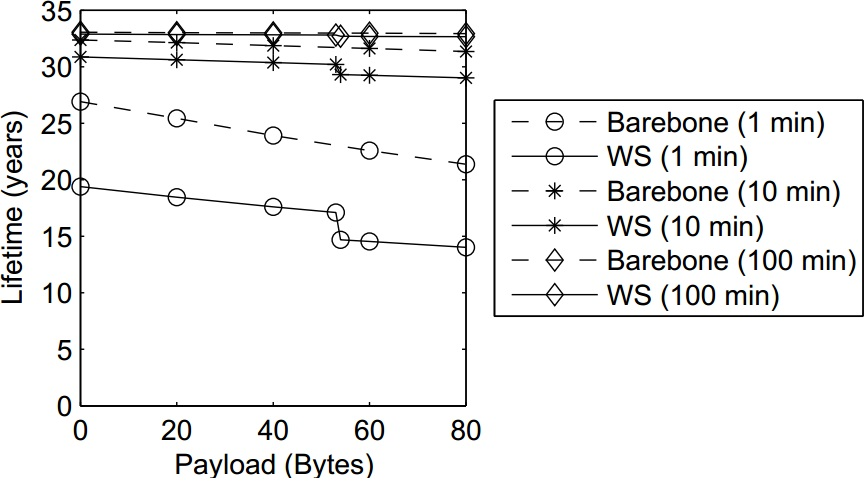
\includegraphics[scale=\radiosca]{figures/radiooff.jpg}
  \caption{Radio éteinte entre les transferts}
 \end{figure} 
\end{frame}

\begin{frame}
 \frametitle{Temps de vie en fonction du payload}
 \framesubtitle{Radio active pendant tout le transfert TCP}
 \begin{figure}
  \centering
  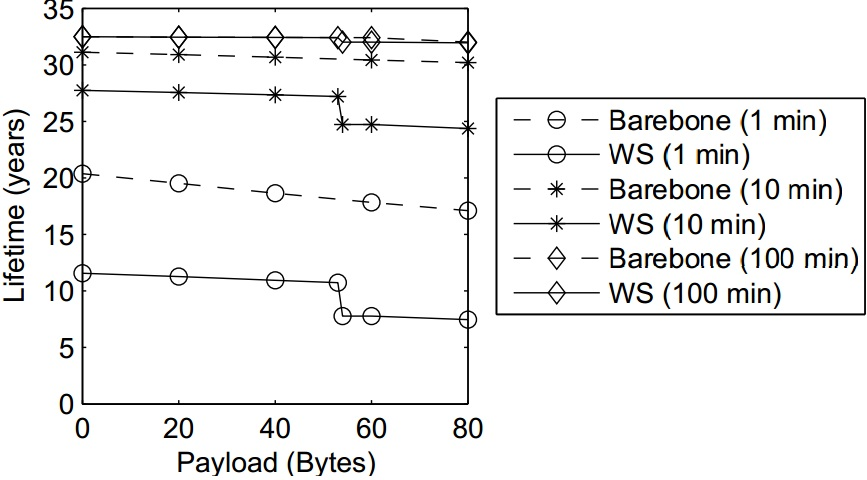
\includegraphics[scale=\radiosca]{figures/radioon.jpg}
  \caption{Radio allumée pendant toute la transmissions}
 \end{figure} 
\end{frame}

\begin{frame}
 \frametitle{Temps de vie en fonction du payload}
 \framesubtitle{Observations}
 On observe que pour des messages inférieur à 53 octets, la taille a très peu d'impact sur le temps de vie
 (réduction de 4,74\% pour des messages de 40 octets si radio éteinte entre les transferts, 10,85\% sinon).
 C'est surtout la fréquence des messages qui réduit le temps de vie. Mais on remarque que la plupart des applications ont une période moyenne entre 10 et 100 minutes.\\
 \vspace{5mm}
 En excluant les messages de période 1 minute, on observe donc que l'impact de l'overhead est assez négligeable.
 En plus, n'oublions pas que dans la réalité, des pertes de paquets et retransmissions auront lieu.
 Les paquets sans header ne sont donc pas envisageables.
\end{frame}

\subsection{Temps de réponse}
\begin{frame}
 \frametitle{Temps de réponse}
 Pour les paquets utilisés lors de l'expérience sur le temps de vie, le temps de réponse mesure le temps entre l'envoi du paquet et la fin de traitement du paquet dans le capteur.
 Un exemple d'application est de pouvoir allumer une lampe à distance.
 \begin{figure}
  \centering
  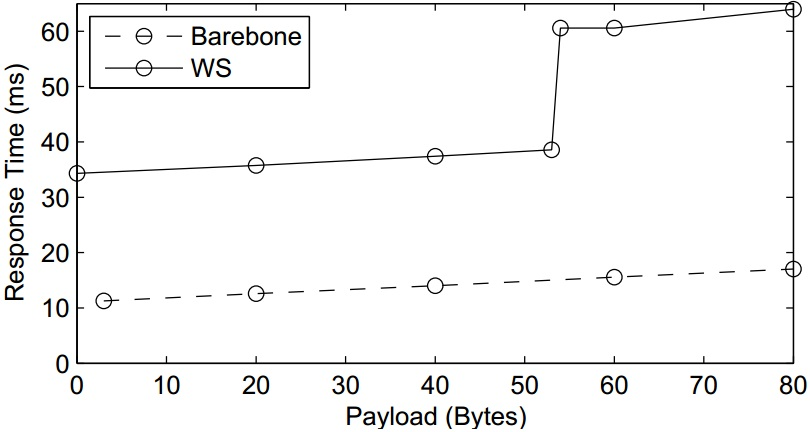
\includegraphics[scale=0.35]{figures/treponse.jpg}
  \caption{Temps de réponse}
 \end{figure} 
\end{frame}
 
\begin{frame}
 \frametitle{Temps de réponse}
 \framesubtitle{Observations}
 Même si le message est envoyé en 2 paquets, le temps de réponse est toujours des quelques dizaines de millisecondes.
 Ce qui est bien suffisamment court pour l'application qu'ils vont en faire.\\
 \begin{block}{Remarque}
 Nous avons vu dans la section précédente que le protocole TCP utilisé envoie un message ACK après chaque réception de paquet.
 Cela explique la forte augmentation de latence lorsque le message est envoyé en 2 paquets.
 Mais nous pouvons réduire cette augmentation en designant un autre protocole TCP qui va envoyé plusieurs paquets sans attendre un ACK entre chaque paquets envoyés ou alors un système de fragmentation/défragmentation sur la couche lien.
 \end{block}
\end{frame}